% Options for packages loaded elsewhere
\PassOptionsToPackage{unicode}{hyperref}
\PassOptionsToPackage{hyphens}{url}
\PassOptionsToPackage{dvipsnames,svgnames,x11names}{xcolor}
%
\documentclass[
  letterpaper,
  DIV=11,
  numbers=noendperiod]{scrartcl}

\usepackage{amsmath,amssymb}
\usepackage{iftex}
\ifPDFTeX
  \usepackage[T1]{fontenc}
  \usepackage[utf8]{inputenc}
  \usepackage{textcomp} % provide euro and other symbols
\else % if luatex or xetex
  \usepackage{unicode-math}
  \defaultfontfeatures{Scale=MatchLowercase}
  \defaultfontfeatures[\rmfamily]{Ligatures=TeX,Scale=1}
\fi
\usepackage{lmodern}
\ifPDFTeX\else  
    % xetex/luatex font selection
\fi
% Use upquote if available, for straight quotes in verbatim environments
\IfFileExists{upquote.sty}{\usepackage{upquote}}{}
\IfFileExists{microtype.sty}{% use microtype if available
  \usepackage[]{microtype}
  \UseMicrotypeSet[protrusion]{basicmath} % disable protrusion for tt fonts
}{}
\makeatletter
\@ifundefined{KOMAClassName}{% if non-KOMA class
  \IfFileExists{parskip.sty}{%
    \usepackage{parskip}
  }{% else
    \setlength{\parindent}{0pt}
    \setlength{\parskip}{6pt plus 2pt minus 1pt}}
}{% if KOMA class
  \KOMAoptions{parskip=half}}
\makeatother
\usepackage{xcolor}
\setlength{\emergencystretch}{3em} % prevent overfull lines
\setcounter{secnumdepth}{-\maxdimen} % remove section numbering
% Make \paragraph and \subparagraph free-standing
\makeatletter
\ifx\paragraph\undefined\else
  \let\oldparagraph\paragraph
  \renewcommand{\paragraph}{
    \@ifstar
      \xxxParagraphStar
      \xxxParagraphNoStar
  }
  \newcommand{\xxxParagraphStar}[1]{\oldparagraph*{#1}\mbox{}}
  \newcommand{\xxxParagraphNoStar}[1]{\oldparagraph{#1}\mbox{}}
\fi
\ifx\subparagraph\undefined\else
  \let\oldsubparagraph\subparagraph
  \renewcommand{\subparagraph}{
    \@ifstar
      \xxxSubParagraphStar
      \xxxSubParagraphNoStar
  }
  \newcommand{\xxxSubParagraphStar}[1]{\oldsubparagraph*{#1}\mbox{}}
  \newcommand{\xxxSubParagraphNoStar}[1]{\oldsubparagraph{#1}\mbox{}}
\fi
\makeatother


\providecommand{\tightlist}{%
  \setlength{\itemsep}{0pt}\setlength{\parskip}{0pt}}\usepackage{longtable,booktabs,array}
\usepackage{calc} % for calculating minipage widths
% Correct order of tables after \paragraph or \subparagraph
\usepackage{etoolbox}
\makeatletter
\patchcmd\longtable{\par}{\if@noskipsec\mbox{}\fi\par}{}{}
\makeatother
% Allow footnotes in longtable head/foot
\IfFileExists{footnotehyper.sty}{\usepackage{footnotehyper}}{\usepackage{footnote}}
\makesavenoteenv{longtable}
\usepackage{graphicx}
\makeatletter
\def\maxwidth{\ifdim\Gin@nat@width>\linewidth\linewidth\else\Gin@nat@width\fi}
\def\maxheight{\ifdim\Gin@nat@height>\textheight\textheight\else\Gin@nat@height\fi}
\makeatother
% Scale images if necessary, so that they will not overflow the page
% margins by default, and it is still possible to overwrite the defaults
% using explicit options in \includegraphics[width, height, ...]{}
\setkeys{Gin}{width=\maxwidth,height=\maxheight,keepaspectratio}
% Set default figure placement to htbp
\makeatletter
\def\fps@figure{htbp}
\makeatother
% definitions for citeproc citations
\NewDocumentCommand\citeproctext{}{}
\NewDocumentCommand\citeproc{mm}{%
  \begingroup\def\citeproctext{#2}\cite{#1}\endgroup}
\makeatletter
 % allow citations to break across lines
 \let\@cite@ofmt\@firstofone
 % avoid brackets around text for \cite:
 \def\@biblabel#1{}
 \def\@cite#1#2{{#1\if@tempswa , #2\fi}}
\makeatother
\newlength{\cslhangindent}
\setlength{\cslhangindent}{1.5em}
\newlength{\csllabelwidth}
\setlength{\csllabelwidth}{3em}
\newenvironment{CSLReferences}[2] % #1 hanging-indent, #2 entry-spacing
 {\begin{list}{}{%
  \setlength{\itemindent}{0pt}
  \setlength{\leftmargin}{0pt}
  \setlength{\parsep}{0pt}
  % turn on hanging indent if param 1 is 1
  \ifodd #1
   \setlength{\leftmargin}{\cslhangindent}
   \setlength{\itemindent}{-1\cslhangindent}
  \fi
  % set entry spacing
  \setlength{\itemsep}{#2\baselineskip}}}
 {\end{list}}
\usepackage{calc}
\newcommand{\CSLBlock}[1]{\hfill\break\parbox[t]{\linewidth}{\strut\ignorespaces#1\strut}}
\newcommand{\CSLLeftMargin}[1]{\parbox[t]{\csllabelwidth}{\strut#1\strut}}
\newcommand{\CSLRightInline}[1]{\parbox[t]{\linewidth - \csllabelwidth}{\strut#1\strut}}
\newcommand{\CSLIndent}[1]{\hspace{\cslhangindent}#1}

\KOMAoption{captions}{tableheading}
\makeatletter
\@ifpackageloaded{caption}{}{\usepackage{caption}}
\AtBeginDocument{%
\ifdefined\contentsname
  \renewcommand*\contentsname{Table of contents}
\else
  \newcommand\contentsname{Table of contents}
\fi
\ifdefined\listfigurename
  \renewcommand*\listfigurename{List of Figures}
\else
  \newcommand\listfigurename{List of Figures}
\fi
\ifdefined\listtablename
  \renewcommand*\listtablename{List of Tables}
\else
  \newcommand\listtablename{List of Tables}
\fi
\ifdefined\figurename
  \renewcommand*\figurename{Figure}
\else
  \newcommand\figurename{Figure}
\fi
\ifdefined\tablename
  \renewcommand*\tablename{Table}
\else
  \newcommand\tablename{Table}
\fi
}
\@ifpackageloaded{float}{}{\usepackage{float}}
\floatstyle{ruled}
\@ifundefined{c@chapter}{\newfloat{codelisting}{h}{lop}}{\newfloat{codelisting}{h}{lop}[chapter]}
\floatname{codelisting}{Listing}
\newcommand*\listoflistings{\listof{codelisting}{List of Listings}}
\makeatother
\makeatletter
\makeatother
\makeatletter
\@ifpackageloaded{caption}{}{\usepackage{caption}}
\@ifpackageloaded{subcaption}{}{\usepackage{subcaption}}
\makeatother

\ifLuaTeX
  \usepackage{selnolig}  % disable illegal ligatures
\fi
\usepackage{bookmark}

\IfFileExists{xurl.sty}{\usepackage{xurl}}{} % add URL line breaks if available
\urlstyle{same} % disable monospaced font for URLs
\hypersetup{
  pdftitle={COVID-19 Pandemic in the US},
  pdfauthor={Irisa Jin, Xu Han, Cenjia Zeng},
  colorlinks=true,
  linkcolor={blue},
  filecolor={Maroon},
  citecolor={Blue},
  urlcolor={Blue},
  pdfcreator={LaTeX via pandoc}}


\title{COVID-19 Pandemic in the US}
\author{Irisa Jin, Xu Han, Cenjia Zeng}
\date{}

\begin{document}
\maketitle


\section{Abstract}\label{abstract}

This study focuses on the COVID-19 pandemic's impact in the United
States from January 2020 to December 2024, especially on temporal and
geographic mortality patterns, changes in the virus's virulence, and the
relationship between COVID-19 mortality and excess mortality. The
pandemic was divided into three distinct periods---the initial outbreak,
the Delta variant surge, and the Omicron wave---based on visualized
trends in cases and mortality. State-level mortality rates were computed
for each period, which identifies states that performed better or worse
in managing the pandemic. Trends in hospitalization and mortality rates
were analyzed across the three periods to evaluate changes in virulence.
The Delta variant exhibited higher virulence with elevated mortality
rates, while the Omicron wave showed reduced severity due to widespread
vaccination and improved treatments. Excess mortality was estimated
weekly for each state, comparing observed and estimated mortality
trends. Regression analysis revealed a strong and statistically
significant relationship between COVID-19 mortality and excess
mortality, further validated through visual alignments. However,
discrepancies in early data and under reporting in later stages
introduced uncertainties. This analysis emphasizes the importance of
vaccination campaigns, targeted public health interventions, and
addressing systemic inequities. These findings provide valuable
suggestions to improve pandemic preparedness and reduce disparities in
future health crises.

\section{Introduction}\label{introduction}

The COVID-19 pandemic has deeply impacted global health and mortality,
displaying some vulnerabilities in healthcare systems worldwide.
Official statistics report millions of deaths, but evidence suggests the
actual toll is 1.6 times higher than reported due to underreporting and
the indirect effects of the pandemic (Karlinsky \& Kobak, 2021; Shang et
al., 2022). Excess mortality, the difference between observed and
expected deaths, has become a critical measure for understanding the
pandemic's full impact. This metric includes both direct effects, such
as deaths caused by the virus, and indirect consequences, like delayed
medical care and strained healthcare systems (Kung et al., 2020). By
offering a comprehensive view, excess mortality can guide public health
policies and improve preparedness for future crises (Araja, 2022; Bech
et al., 2021).

Globally, the impact of COVID-19 on mortality has varied. Some regions,
like South America and parts of Asia, experienced high excess mortality
due to severe outbreaks and healthcare challenges (Shang et al., 2022).
In contrast, other areas saw reductions in non-COVID deaths, as measures
like lockdowns limited the spread of other infectious diseases
(Karlinsky \& Kobak, 2021). In the United States, the pandemic showed
significant health disparities. African American and Hispanic
communities suffered disproportionately high death rates, largely due to
structural inequalities like limited healthcare access and economic
barriers (Siegel et al., 2021; Goldstein \& Atherwood, 2020). These
inequities underscore the importance of state-level analyses to identify
patterns and develop equitable health interventions (Kung et al., 2020).

Evidence suggests that COVID-19 became less severe over time in some
populations. For instance, by early 2022, case-hospitalization rates had
decreased by 90\% in locations like Spain and Boston compared to the
start of the pandemic (Amer et al., 2022). Similarly, Massachusetts
healthcare workers experienced fewer severe complications after April
2020 (Lan et al., 2020). Nationwide U.S. data from April 2020 to April
2021 showed that severe cases were a minority of hospital admissions,
with their proportion decreasing over time (Whitfield et al., 2021).
However, these improvements were not evenly distributed. Vulnerable
groups, including racial and ethnic minorities, older adults, and
socioeconomically disadvantaged populations, continued to experience
higher rates of severe illness and death (Bergmann et al., 2022). This
emphasizes the need to study changes in COVID-19 severity across
different waves and populations to introduce adaptive public health
strategies.

This study aims to analyze mortality trends in the United States from
January 2020 to December 2024. Using daily and weekly mortality data, it
will divide the pandemic into distinct waves based on trends observed
through data visualizations. For each wave, the study will show the
calculation of state-level death rates to identify which states were
most and least affected. It will also assess whether COVID-19 became
less severe over time by examining hospitalization and death rates.
Additionally, this study will estimate weekly excess mortality for each
state and evaluate how much of it can be attributed to COVID-19 deaths.
By exploring both COVID-19-related and unrelated mortality, this study
seeks to provide a clearer picture of the pandemic's full impact.
Through careful analysis and visualization, the study's findings aim to
inform public health strategies and improve readiness for future health
emergencies (Ramírez-Soto \& Ortega-Cáceres, 2022; Stokes et al., 2021).

\section{Methods}\label{methods}

The data used in this project are from multiple sources, including
COVID-19 cases, deaths, hospitalizations, and vaccination records from
CDC APIs, state-level population estimates from the US Census Bureau,
and state-to-region mappings from publicly available JSON files. The
estimated mortality was built based on the 2014-2019 mortality data
which was sourced from CDC. Specifically, the time series approach was
implemented by using state-level total death with 52 weeks per year.
However, it was found that 2014 had 53 weeks which was considered as an
outlier and was omitted from the analysis. The ARIMA model was used for
fitting procedures in order to identify patterns and seasonality. A
208-week data frame was generated to forecast 2020 - 2023
mortality-related data. The results were aggregated to produce estimated
mortality for each state without interruption from the COVID pandemic.
The main data preprocessing involved cleaning, aggregating, and joining
datasets by state and week using the CDC's MMWR format and saved into
``dat'' data frame in the ``WrangledData.rdata'' file. Rates per 100,000
people were calculated for comparability across states and time periods.
Then, the estimated data was merged with ``dat'' by year, week, and
state. Later analysis was conducted based on these cleaned data. All
programming was conducted in the R language. When dividing wave periods,
data visualization packages were used to examine the data. The
visualized graphs depicted a peak sandwiched between two flat zones;
this was considered the epidemic wave. The pandemic was divided into
three periods with more accurate time nodes based on time-series trends
publish by the CDC: (1) starting from the initial global outbreak (Jan
25, 2020 -- Feb 28, 2021), characterized by the first significant wave
of COVID-19; (2) the beginning of the Delta Variant Surge (Mar 1, 2021
-- Nov 30, 2021), marked by a rise in cases and deaths associated with
the Delta variant; and (3) seeing the Omicron wave (Dec 1, 2021 -- Apr
29, 2023), notable for a sharp increase in cases but a lower mortality
rate due to widespread vaccinations.

State-level death rates were calculated for each period, and trends in
hospitalization and death rates were analyzed to assess changes in
virulence over time. Visualizations, including time-series plots and bar
charts, were created using ggplot2 to support these analyses.

To test the relationship between COVID-19 and the excess mortality, the
linear regression was conducted to examine the association between the
COVID-related mortality and the excess mortality. To make the results
more visible, a scatter plot with fitted lines was generated. A box plot
visualizes the distribution of excess deaths across states, highlighting
the median, interquartile range, and potential outliers, which helps
identify variability and patterns in excess deaths and provides insight
into the excess mortality in different states. The box plot also
supports hypothesis testing and comparisons among states. A line chart
was used to look at how well the actual number of mortality and the
number of estimated deaths plus the number of COVID deaths fit. The
closer fitted lines represent more similar trends, indicating that COVID
may be used to explain excess mortality.

Lastly, the above processes regarding states' performance in COVID were
repeated for excess mortality. After separating the results by state,
the weekly average mortality rate and total mortality rate were
examined. The rate calculations were based on rate per 100,000 people.

\section{Results}\label{results}

The COVID-19 pandemic was divided into three periods based on the
observed trends in case and death rates across the US states, as well as
outside information. From Figure 1, three major peaks were defined to be
both present in case and death rate. They corresponded to and included
the initial global outbreak, Delta Variant surge, and the Omicron wave;
this was matched to information given by the official CDC website. The
initial global outbreak (Jan 25, 2020 -- Feb 28, 2021) is marked by the
first large peak in cases and deaths, with a steep rise in both metrics
during late 2020 and early 2021. The Delta Variant surge (Mar 1, 2021 --
Nov 30, 2021) shows a distinct increase in both case and death rates,
albeit with a broader and steady peak. Lastly, the Omicron wave (Dec 1,
2021 -- Apr 29, 2023) features a sharp, high spike in case rates but a
comparatively smaller rise in death rates, suggesting a shift in the
pandemic dynamics and the advancements in scientific discoveries
(widespread of vaccines).

State-level death rates varied significantly across the defined periods.
From Figure 2, it can be clearly seen that in period (1), states like
Rhode Island, New Jersey, and Mississippi reported the highest death
rates, reflecting the early and severe impact of the pandemic in these
regions, with Vermont and Hawaii at the lowest death rates. During the
(2) phase, West Virginia, Florida, and Tennessee experienced the highest
death rates, while Vermont, New Hampshire, and Rhode Island showed the
lowest death rates. In (3) time period, West Virginia, Kentucky, and
Ohio had the highest death rates, while Alaska, Hawaii, and Vermont had
the lowest death rates. Interestingly, Vermont, Hawaii, and Alaska
remains having the lowest death rates throughout the pandemic, possibly
due to a small population and less ability to spread the disease.

The virulence of COVID-19 appeared to decrease over time, as evidenced
by Figure 3. In (1), the vaccination (regular and booster, which has not
been available yet) remains to be almost 0; the hospitalization rate
increases rapidly in this time period. In (2), the regular series is
increasing and people also begin to take booster vaccines; the
hospitalization rate is not as high as (1). There is a large peak of
hospitalization in (3) but declines quickly, possibly due to high
vaccination (including booster) rates. This conclusion can also be
explained by a decreasing death rate.

The time series analysis produced estimated data for 2020 - 2023 as
expected. The result from linear regression is shown in Table 1. From
the result, the excess mortality can be explained by the COVID pandemic.
The LINE assumptions check passed by checking Q-Q plot and residual
plot. A scatterplot was used to more clearly depict the relationship
between the variables. It can be seen in the scatterplot that the dots
form a straight line. In the Figure 4, it can also be seen that when
COVID mortality was added to the actual mortality, it was very close to
the estimated mortality, especially in 2020 - 2022.~

State-level excess death rates varied significantly across the defined
periods. A more negative excess mortality rate represents a larger rate.
From Figure 2, it can be clearly seen that in period (1), states like
Mississippi, Arizona, and Louisiana reported the highest excess death
rates, with Vermont and Hawaii at the lowest death rates. During the (2)
phase, West Virginia, Florida, and Montana experienced the highest
excess death rates, while Massachusetts, District of Columbias and
Minnesota showed the lowest excess death rates. In (3) time period, West
Virginia, New Mexico, and Puerto Rico had the highest death rates, while
District of Columbia, New Jersey, and Minnesota had the lowest death
rates. Unlike results found for question two, no states remained having
consistently the lowest death rate.

\begin{figure}[H]

{\centering 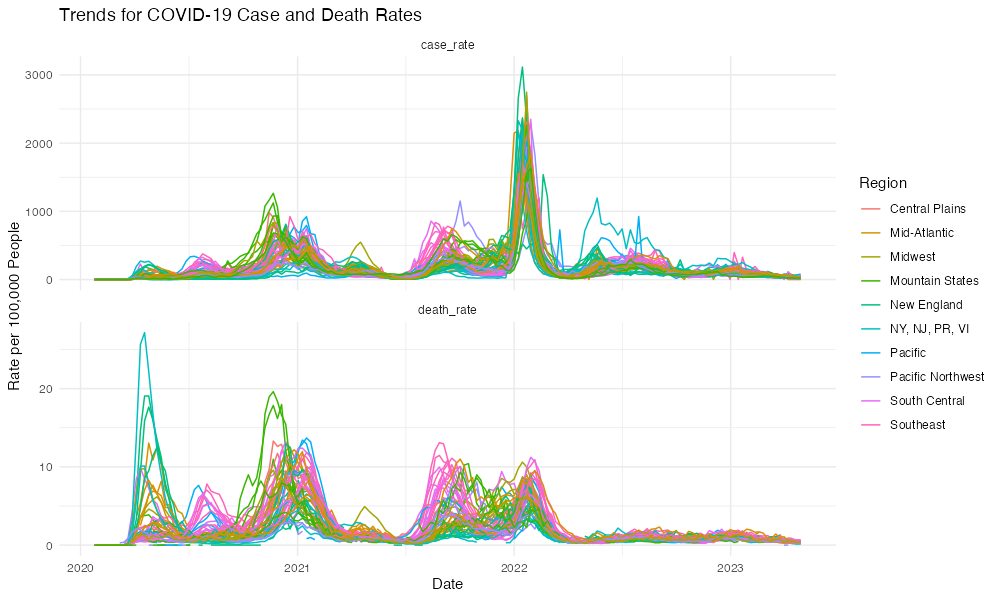
\includegraphics{../docs/covid_state_region.png}

}

\caption{COVID of State and Region}

\end{figure}%%
\begin{figure}[H]

{\centering 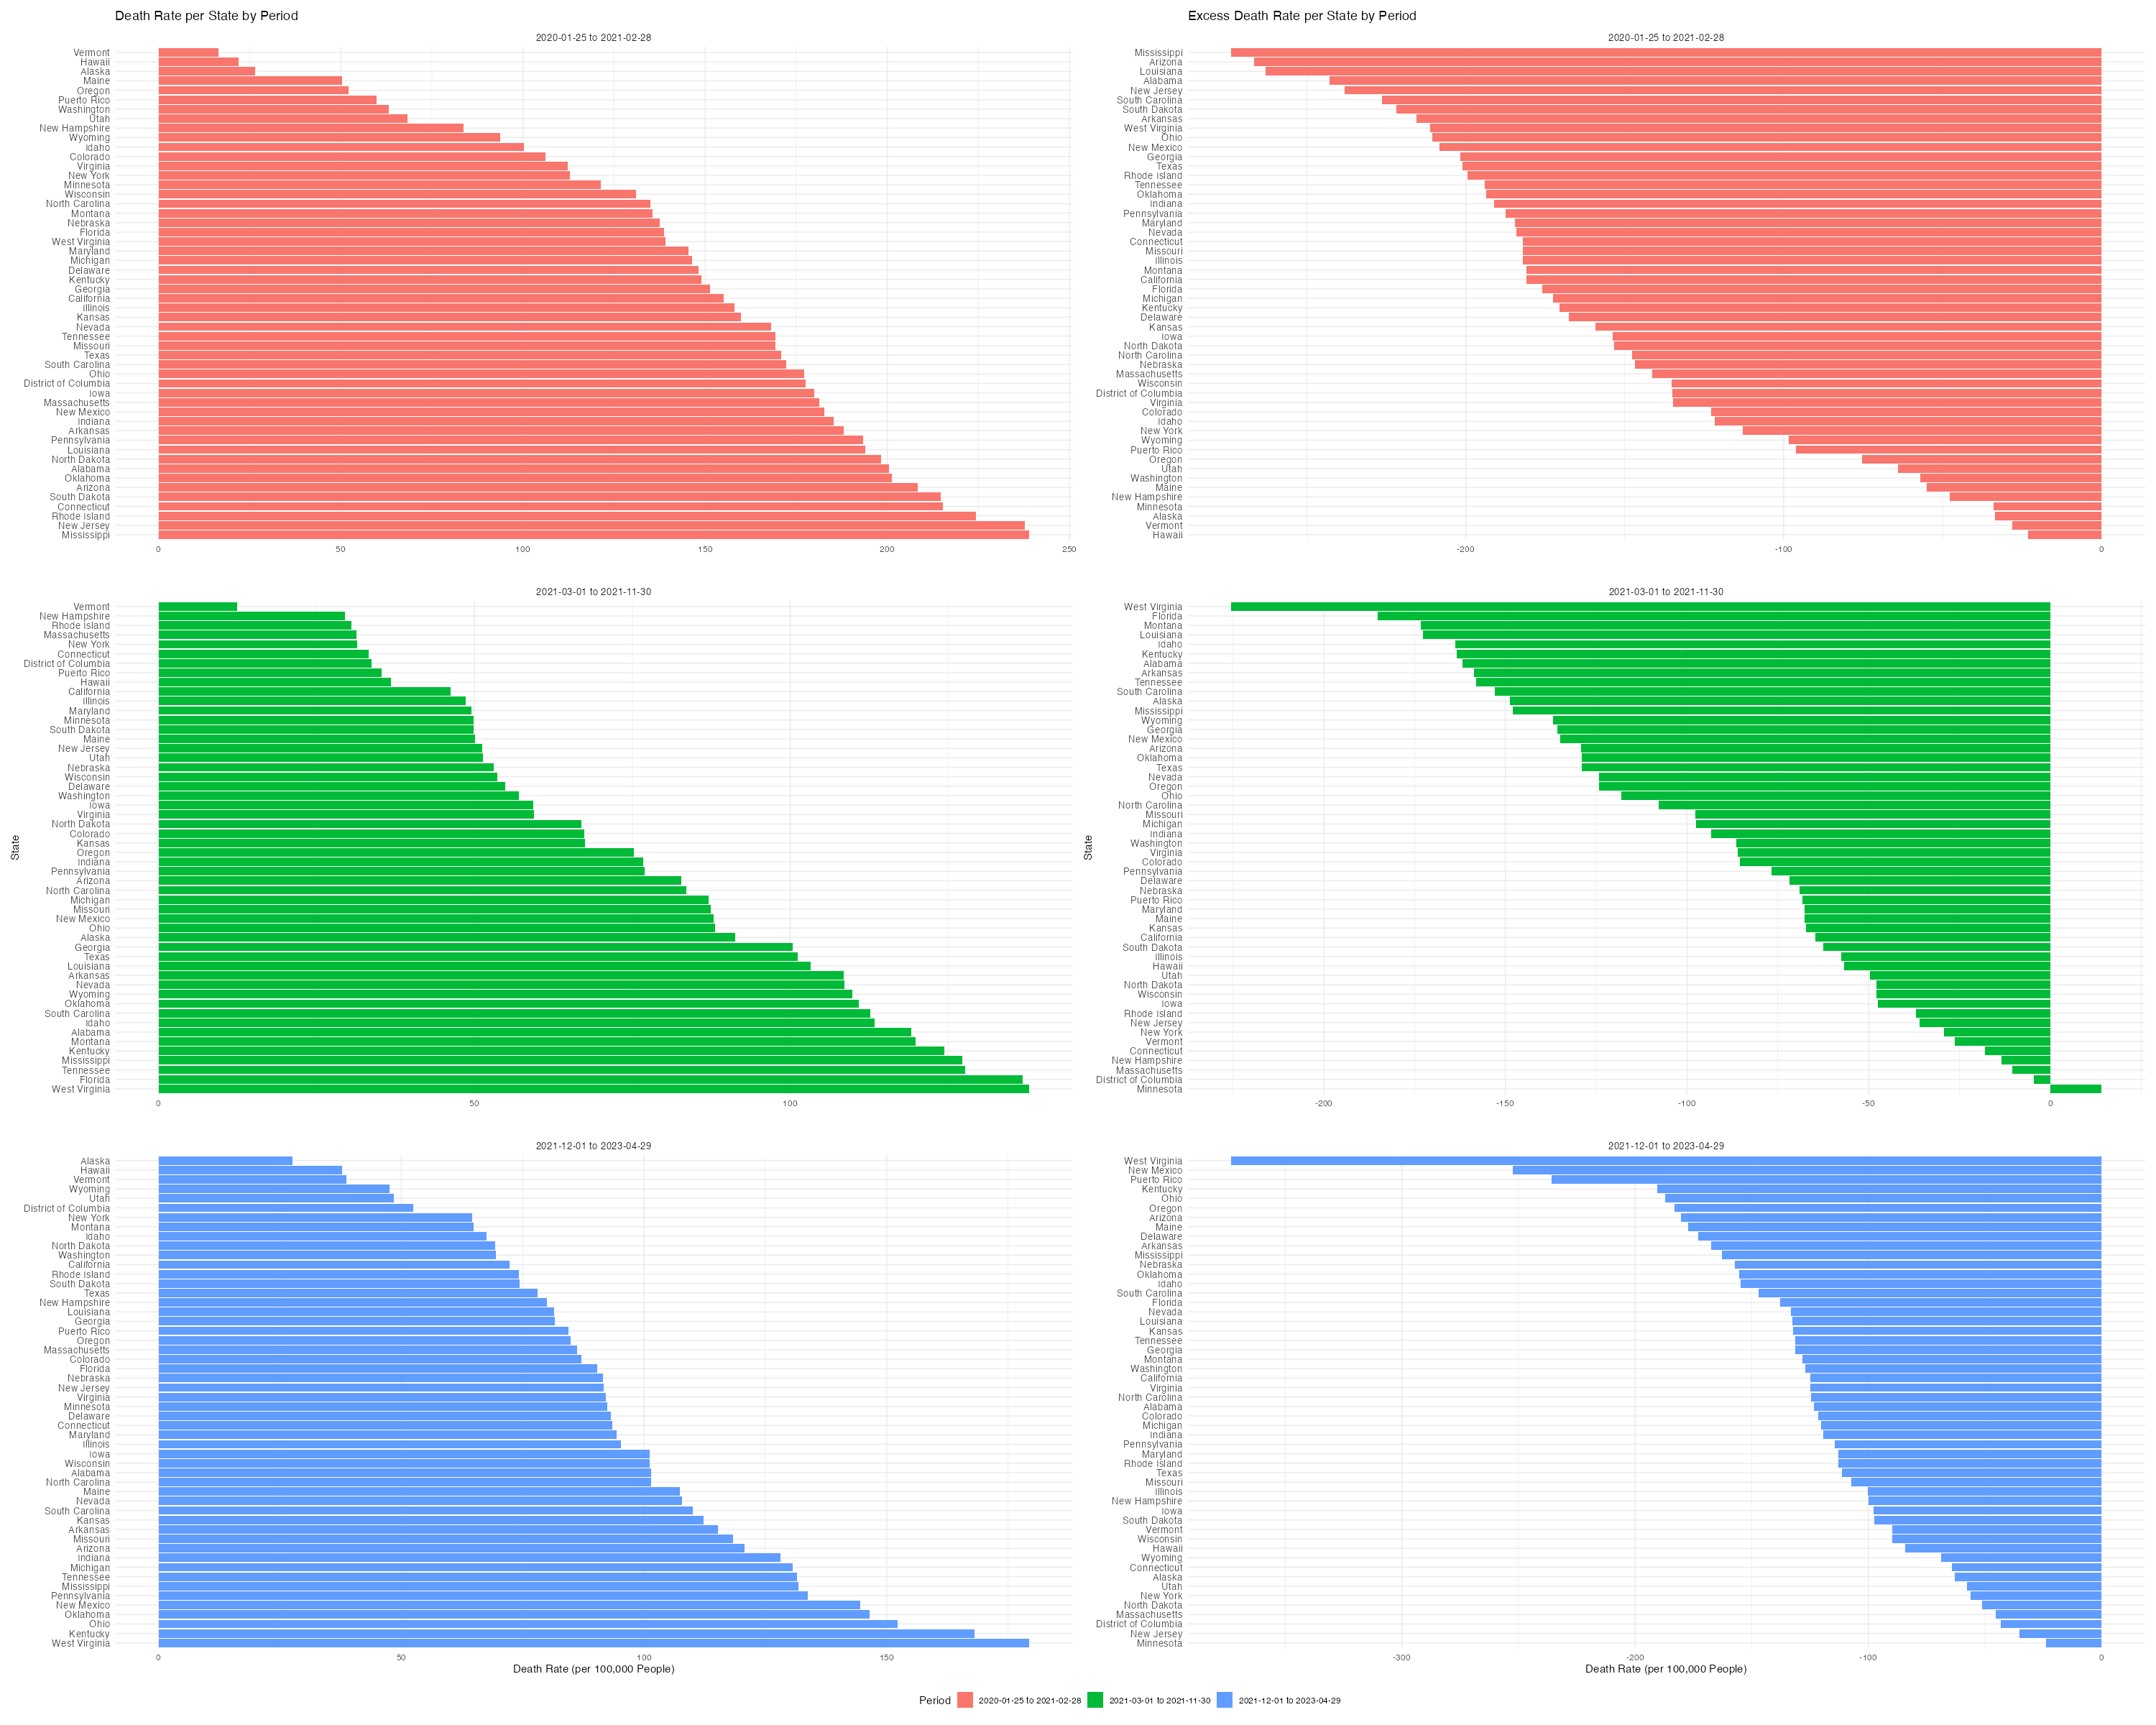
\includegraphics{images/excess_death_by_state.png}

}

\caption{COVID and Excess Death by State}

\end{figure}%%
\begin{figure}[H]

{\centering 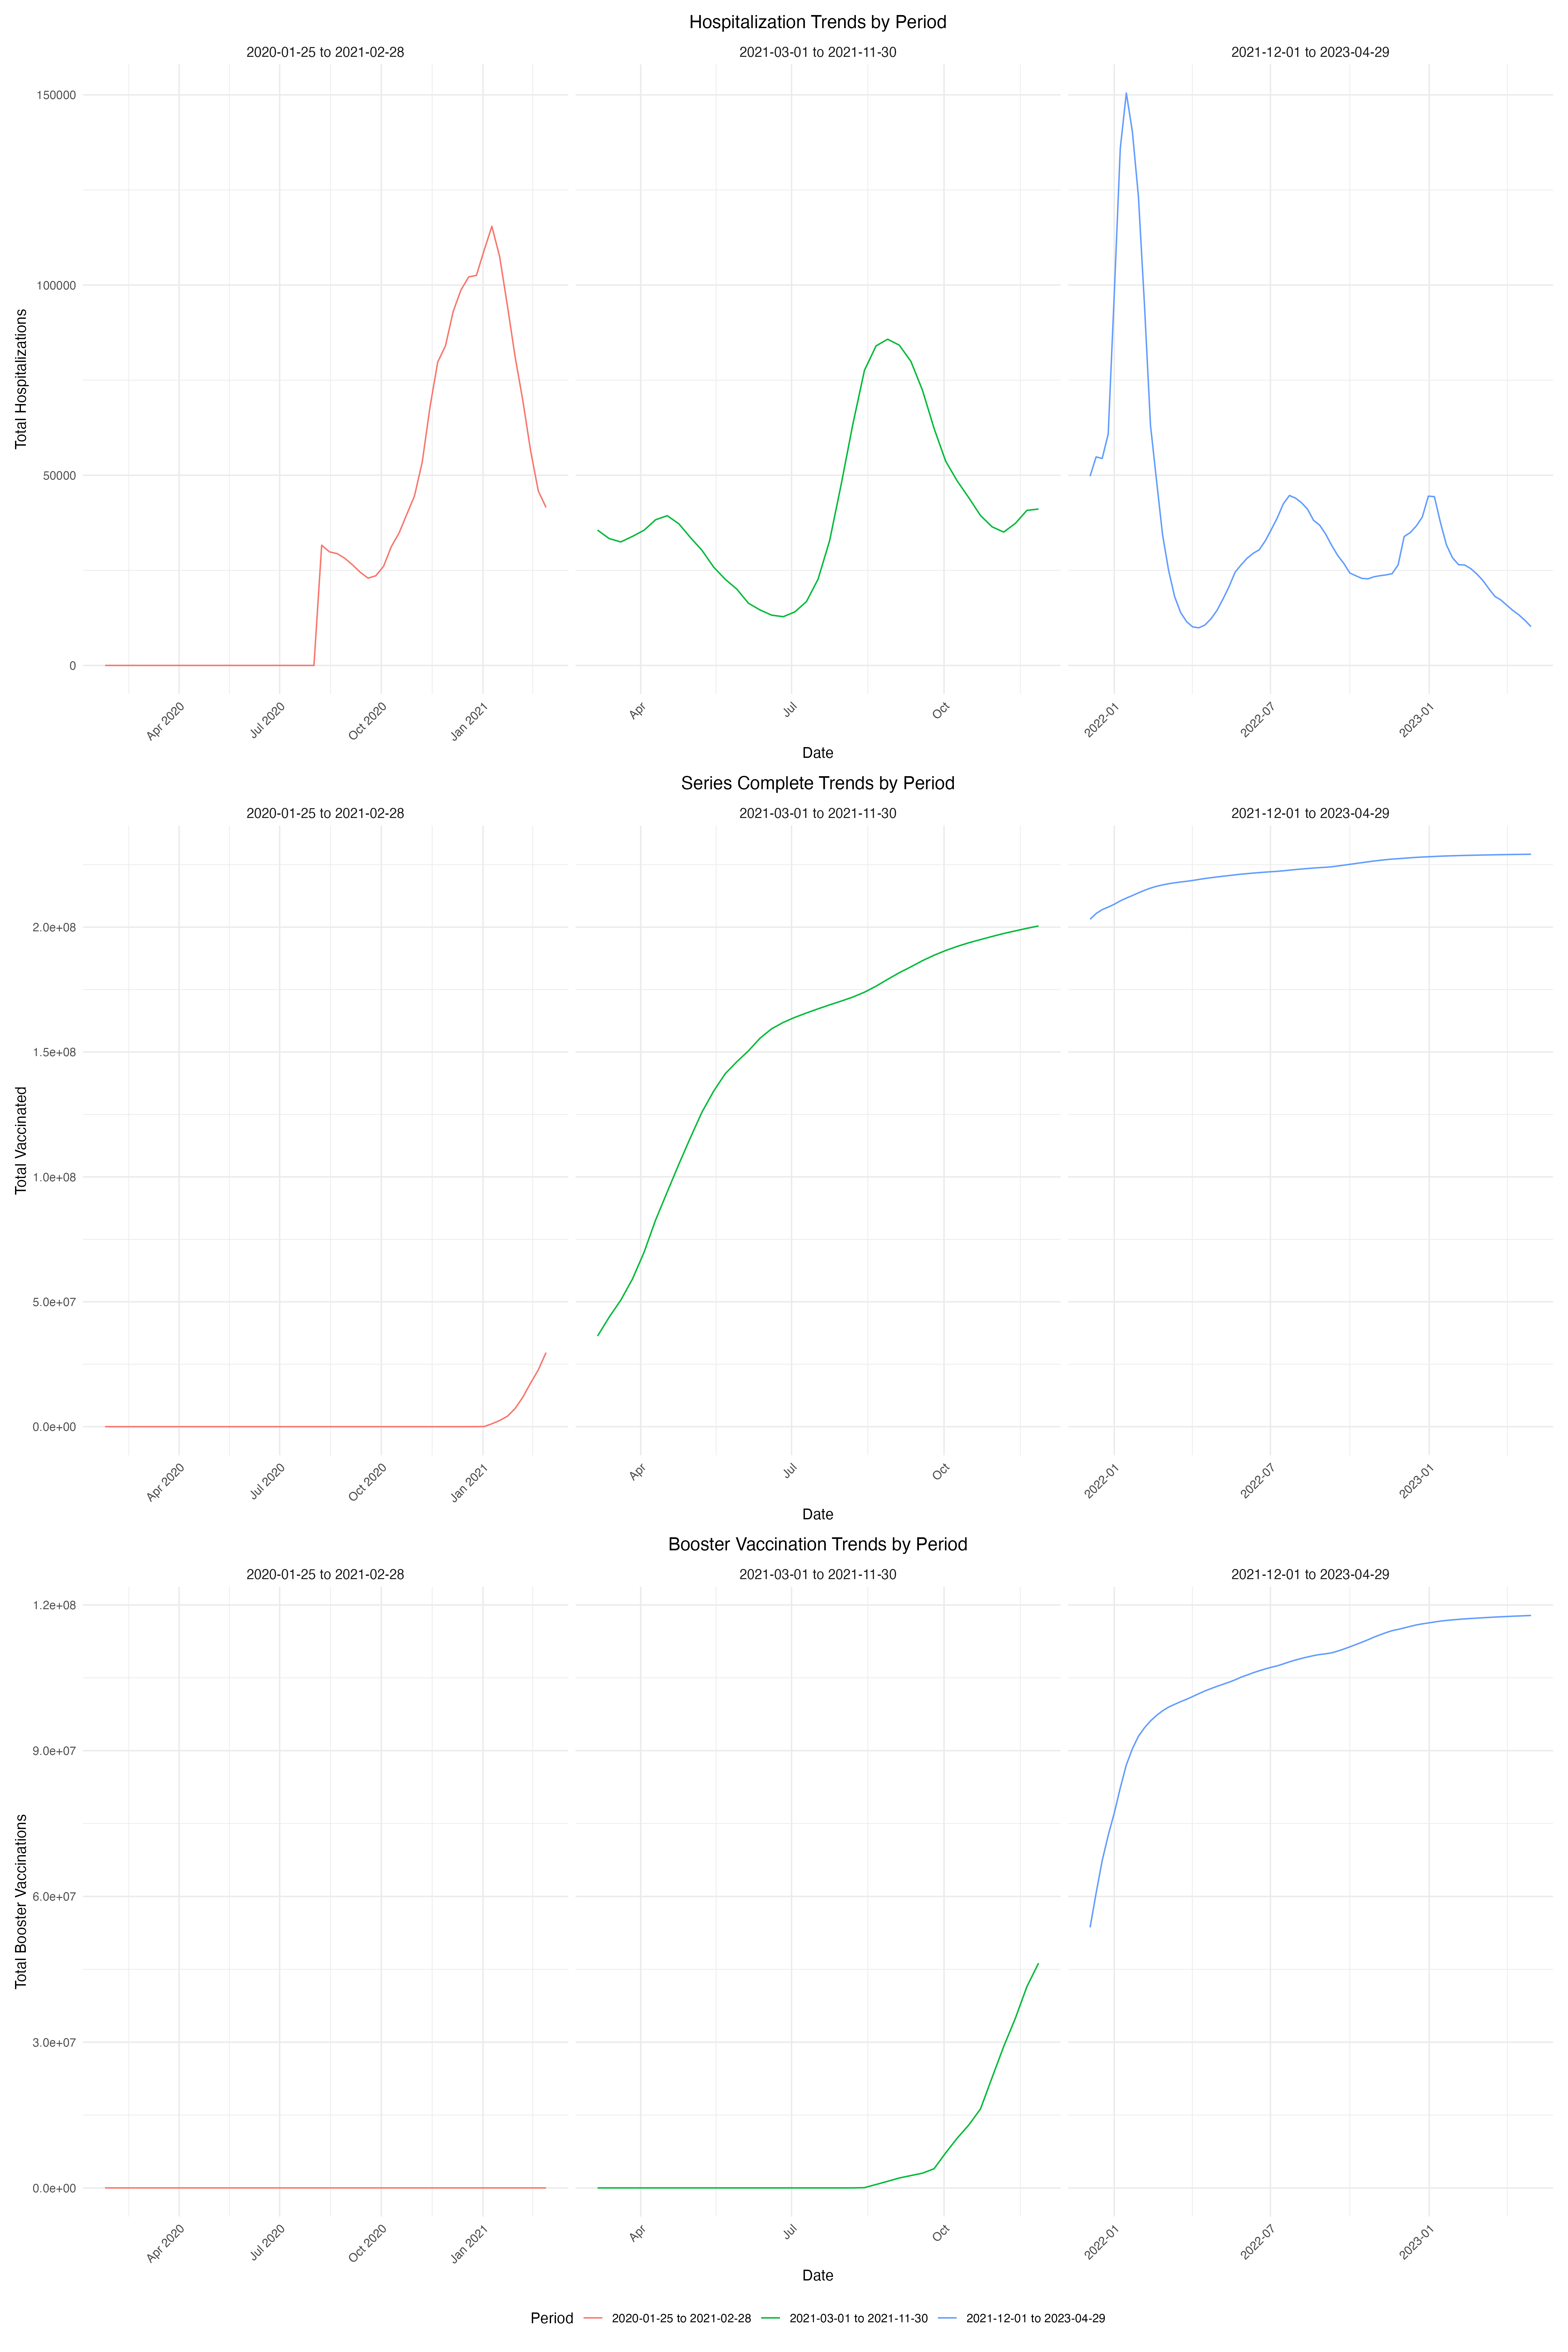
\includegraphics{../docs/stacked.png}

}

\caption{Hospitalization \& Series Complete \& Booster}

\end{figure}%%
\begin{figure}[H]

{\centering 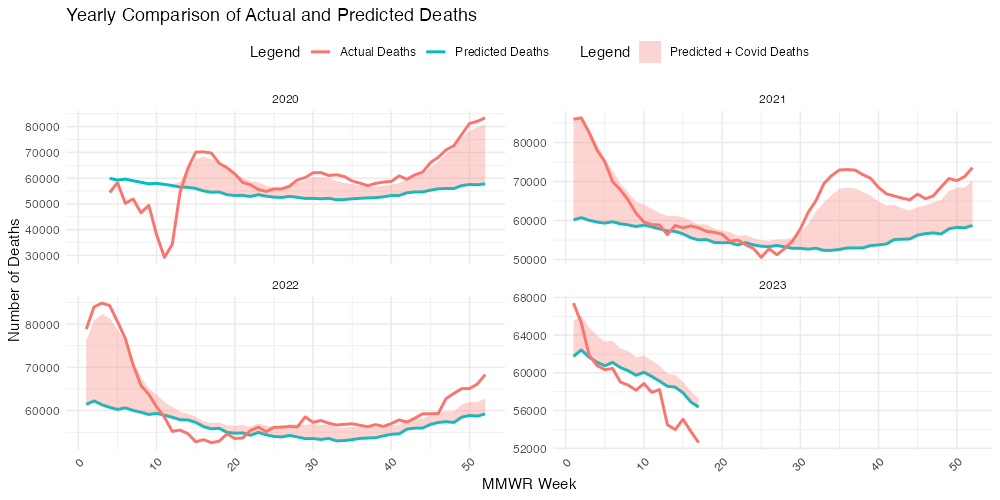
\includegraphics{../docs/yearly_comparison_of_actual_and_predicted_deaths.png}

}

\caption{Line Chart: Yearly Comparison}

\end{figure}%

\begin{longtable}[]{@{}l@{}}
\caption{Linear Regression Summary}\tabularnewline
\toprule\noalign{}
\endfirsthead
\endhead
\bottomrule\noalign{}
\endlastfoot
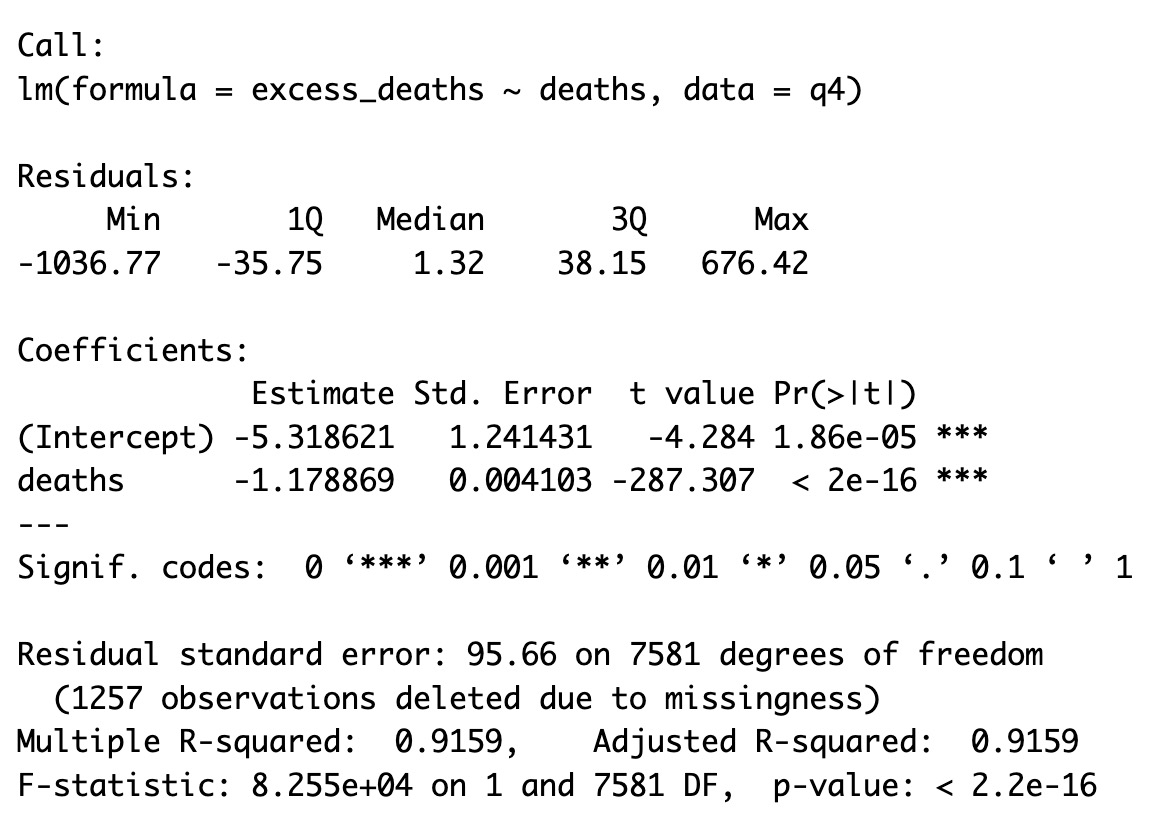
\includegraphics{../docs/table1.jpg} \\
\end{longtable}

\section{Discussion}\label{discussion}

This study's analysis of the COVID-19 pandemic in the United States
provides valuable insights into the shifting patterns of cases,
mortality, and the virus's overall impact over time. By dividing the
pandemic into three major periods---initial outbreak, Delta variant
surge, and Omicron wave---this study captured critical temporal and
geographic variations, along with changes in the COVID-19's virulence.
These findings align with existing research while offering new opinions
on public health strategies.

\textbf{Temporal Trends and Pandemic Waves}

Dividing the pandemic into three waves revealed how the challenges posed
by COVID-19 evolved. The initial outbreak was noticed by steep increases
in both cases and mortality. This reflects a lack of preparedness and
natural immunity early in the pandemic. This phase indicated significant
stress on healthcare systems nationwide. And it had broader observations
of overwhelmed resources and elevated mortality rates during the first
months of the pandemic.

The Delta variant surge maintained high mortality rates, which
emphasizes variant's increased virulence compared to the original
strain. This finding aligns with existing research showing higher
hospitalization and mortality rates during Delta than in other phases of
the pandemic (Li et al., 2023). In contrast, the Omicron wave brought a
record surge in cases but a comparatively smaller rise in mortality.
This trend reflects the widespread impact of vaccination and improved
treatments, which were critical in mitigating severe outcomes despite
higher transmission rates (Lin et al., 2022). Vaccination campaigns
likely reduced mortality by up to 70\% during the Delta wave, displaying
their importance in changing the trajectory of the pandemic.

These patterns explain how targeted public health interventions, such as
timely vaccine rollouts, can influence pandemic outcomes. However, they
also emphasize that a uniform strategy may not be enough because
distinct waves presented different challenges across time and regions.

\textbf{Geographic and State-Level Variations}

Significant disparities in mortality rates across states persisted
throughout the pandemic. States such as West Virginia and Kentucky
consistently reported higher mortality rates, while Vermont and Hawaii
maintained the lowest rates. This disparity reflects a range of factors,
including population density, healthcare capacity, and demographic
vulnerabilities. For instance, Vermont's lower population density likely
reduced transmission risks, while states with weaker healthcare systems
faced greater difficulties managing surges.

Additionally, structural inequities, such as systemic racism, further
exacerbated these disparities. Black and Hispanic populations faced
disproportionately high mortality rates, even after adjusting for other
factors (Goldstein \& Atherwood, 2020; Sehra et al., 2020). These
findings indicate the need for targeted interventions to address
underlying systemic inequities, such as expanding healthcare access and
addressing socioeconomic barriers in vulnerable communities.

\textbf{Declining Virulence Over Time}

Trends in hospitalization and mortality rates suggest COVID-19 became
less virulent over time. The significant reduction in mortality rates
during the Omicron wave reflects the success of vaccination campaigns in
preventing severe outcomes. These findings are consistent with research
indicating that vaccines effectively reduce disease severity and
hospitalization rates, even with emerging variants (Lin et al., 2022).
However, vaccines were less effective at preventing transmission. This
emphasizes the importance of developing updated vaccines tailored to new
variants (Krause et al., 2021).

Although some models have suggested that imperfect vaccines could drive
the evolution of more severe strains (Gandon et al., 2001), current
evidence indicates that COVID-19 vaccines have played a key role in
transitioning the virus toward endemicity. Studies have shown that over
time, immunity gained from vaccination and previous infections has
contributed to the decreasing severity of COVID-19 cases (Lavine et al.,
2021).

\textbf{Excess Mortality and COVID-19 Mortality}

The statistical analysis (Table 1) shows an extremely strong and
statistically significant relationship between COVID-19 mortality and
excess mortality, as evidenced by low p-values and high adjusted
R-squared values. This result supports the hypothesis that COVID-19
mortality is closely connected with the gap between estimated and
observed mortality. In other words, COVID-19 mortality aligns well with
the ``excess mortality'' observed during the pandemic.

Figure 4 visually supports this conclusion. The pink shaded area
represents COVID-19 mortality, while the green line indicates estimated
mortality under non-pandemic conditions. The actual mortality (red line)
consistently exceeds the estimated mortality, and the difference aligns
closely with COVID-19 mortality. This alignment indicates that COVID-19
mortality explains much of the observed excess mortality, which
validates the regression results.

However, the model's fit deteriorates in 2023 as the pandemic subsided,
reducing COVID-19's impact on overall mortality and weakening the direct
relationship between COVID-19 and excess mortality. Additionally, data
discrepancies in early 2020, due to missing values in major states'
total mortality records in CDC data, introduced uncertainty. For
example, incomplete data led to artificially low estimates in certain
periods, explaining the discrepancies observed during the early stages
of the pandemic.

\textbf{Implications for Policy and Future Research}

The findings from this study emphasize the need for sustained public
health efforts to address disparities and enhance preparedness for
future pandemics. Policies must prioritize vulnerable populations and
regions with limited healthcare resources. Integrating vaccination
campaigns with public education, equitable resource distribution, and
expanded healthcare access is essential to address these challenges
effectively.

Future research should delve deeper into the interplay between
demographic factors, healthcare access, and policy interventions.
Granular analyses, such as county-level studies, could provide more
localized insights into urban-rural disparities and specific
vulnerabilities. Additionally, long-term research on immunity and the
effectiveness of multivalent vaccines will be critical for shaping
strategies to combat emerging variants in future pandemics.

\textbf{Limitations}

This study offers a comprehensive analysis of COVID-19 trends but has
notable limitations. First, missing CDC data from early 2020,
particularly in major states, introduced extreme outliers, complicating
accurate estimates of excess mortality. Second, as the pandemic waned in
2023, underreporting likely increased as unrecognized or unreported
COVID-19 cases reduced the accuracy of mortality data, weakening the
observed link between COVID-19 and excess mortality. Finally, while the
linear regression model satisfied key assumptions (LINE), Q-Q plots
revealed deviations at the tails, indicating difficulty in capturing
extreme values and potentially affecting the robustness of conclusions
in outlier states.

\textbf{Conclusion}

In conclusion, this study emphasizes the dynamic nature of the COVID-19
pandemic, with significant variations across time, geography, and
population groups. Vaccination campaigns were instrumental in reducing
mortality and reducing the virus's impact, but persistent disparities
reveal the need for targeted public health interventions. By addressing
systemic inequities and enhancing preparedness, we can build a more
equitable and effective healthcare system capable of responding to
future health crises.

\newpage

\section*{References}\label{references}
\addcontentsline{toc}{section}{References}

\phantomsection\label{refs}
\begin{CSLReferences}{1}{0}
\bibitem[\citeproctext]{ref-ahmed_united_2020}
Ahmed, Rashid, Mark Williamson, Muhammad Akhter Hamid, and Naila Ashraf.
2020. {``United States County-Level Covid-19 Death Rates and Case
Fatality Rates Vary by Region and Urban Status.''} \emph{Healthcare} 8
(3): 330. \url{https://doi.org/10.3390/healthcare8030330}.

\bibitem[\citeproctext]{ref-amer_evolving_2022}
Amer, Fares, Fan-Yun Lan, Mario Gil-Conesa, Amalia Sidossis, Daniel
Bruque, Eirini Iliaki, Jane Buley, et al. 2022. {``Evolving
{SARS}-{CoV}-2 Virulence Among Hospital and University Affiliates in
{Spain} and {Greater} {Boston}.''} \emph{MedRxiv}, November, 2022--11.
\url{https://doi.org/10.1101/2022.11.28.22282412}.

\bibitem[\citeproctext]{ref-araja_co136_2022}
Araja, D. 2022. {``Co136 Covid-19 Pandemic Indirect Impact on Mortality
Rates.''} \emph{Value in Health} 25 (7): S329--30.
\url{https://doi.org/10.1016/j.jval.2022.04.231}.

\bibitem[\citeproctext]{ref-bech_ux5cux255Bindirect_2021}
Bech, Christine Manic, Joakim Bloch, Jesper Kjærgaard, Stine Lund,
Freddy Karup Pedersen, and Anja Poulsen. 2021.
{``\href{https://www.ncbi.nlm.nih.gov/pubmed/33734073}{{[}{Indirect}
Effects of the {COVID}-19 Pandemic on Mortality of Mothers and Children
in Low- and Middle-Income Countries{]}}.''} \emph{Ugeskrift for Laeger}
183 (11): V12200903.

\bibitem[\citeproctext]{ref-bergmann_county-level_2022}
Bergmann, Philip J., Nathan A. Ahlgren, and Rosalie A. Torres Stone.
2022. {``County-Level Societal Predictors of {COVID}-19 Cases and Deaths
Changed Through Time in the {United} {States}: {A} Longitudinal
Ecological Study.''} Edited by Javier H. Eslava-Schmalbach. \emph{PLOS
Global Public Health} 2 (11): e0001282.
\url{https://doi.org/10.1371/journal.pgph.0001282}.

\bibitem[\citeproctext]{ref-bureau_state_nodate}
Bureau, US Census. n.d. {``State Population Totals and Components of
Change: 2020-2024.''} \emph{Census.gov}. Accessed December 21, 2024.
\url{https://www.census.gov/data/tables/time-series/demo/popest/2020s-state-total.html}.

\bibitem[\citeproctext]{ref-cdc_cdc_2023}
CDC. 2023. {``Cdc Museum Covid-19 Timeline.''} \emph{Centers for Disease
Control and Prevention}.
\url{https://www.cdc.gov/museum/timeline/covid19.html}.

\bibitem[\citeproctext]{ref-doti_model_2020}
Doti, James L. 2020. {``A Model to Explain Statewide Differences in
Covid-19 Death Rates.''} \emph{SSRN Electronic Journal}.
\url{https://doi.org/10.2139/ssrn.3731803}.

\bibitem[\citeproctext]{ref-gandon_imperfect_2001}
Gandon, Sylvain, Margaret J. Mackinnon, Sean Nee, and Andrew F. Read.
2001. {``Imperfect Vaccines and the Evolution of Pathogen Virulence.''}
\emph{Nature} 414 (6865): 751--56.
\url{https://doi.org/10.1038/414751a}.

\bibitem[\citeproctext]{ref-goldstein_improved_2020}
Goldstein, Joshua R., and Serge Atherwood. 2020. {``Improved Measurement
of Racial/Ethnic Disparities in {COVID}-19 Mortality in the {United}
{States}.''} \emph{MedRxiv}, May, 2020--05.
\url{https://doi.org/10.1101/2020.05.21.20109116}.

\bibitem[\citeproctext]{ref-karlinsky_tracking_2021}
Karlinsky, Ariel, and Dmitry Kobak. 2021. {``Tracking Excess Mortality
Across Countries During the {COVID}-19 Pandemic with the {World}
{Mortality} {Dataset}.''} \emph{eLife} 10 (June): e69336.
\url{https://doi.org/10.7554/eLife.69336}.

\bibitem[\citeproctext]{ref-krause_sars-cov-2_2021}
Krause, Philip R., Thomas R. Fleming, Ira M. Longini, Richard Peto,
Sylvie Briand, David L. Heymann, Valerie Beral, et al. 2021.
{``Sars-Cov-2 Variants and Vaccines.''} \emph{New England Journal of
Medicine} 385 (2): 179--86. \url{https://doi.org/10.1056/NEJMsr2105280}.

\bibitem[\citeproctext]{ref-kung_underestimation_2021}
Kung, Stacey, Marjan Doppen, Melissa Black, Irene Braithwaite, Ciléin
Kearns, Mark Weatherall, Richard Beasley, and Nethmi Kearns. 2021.
{``Underestimation of {COVID}-19 Mortality During the Pandemic.''}
\emph{ERJ Open Research} 7 (1): 00766--2020.
\url{https://doi.org/10.1183/23120541.00766-2020}.

\bibitem[\citeproctext]{ref-lan_evolving_2020}
Lan, Fan-Yun, Robert Filler, Soni Mathew, Eirini Iliaki, Rebecca Osgood,
Lou Ann Bruno-Murtha, and Stefanos N. Kales. 2020. {``Evolving
Virulence? {Decreasing} Covid-19 Complications Among Massachusetts
Healthcare Workers: A Cohort Study.''}
\url{https://doi.org/10.1101/2020.08.17.20176636}.

\bibitem[\citeproctext]{ref-lavine_immunological_2021}
Lavine, Jennie S., Ottar N. Bjornstad, and Rustom Antia. 2021.
{``Immunological Characteristics Govern the Transition of {COVID}-19 to
Endemicity.''} \emph{Science} 371 (6530): 741--45.
\url{https://doi.org/10.1126/science.abe6522}.

\bibitem[\citeproctext]{ref-li_chronological_2023}
Li, Jing-Xing, Pei-Lun Liao, James Cheng-Chung Wei, Shu-Bai Hsu, and
Chih-Jung Yeh. 2023. {``A Chronological Review of {COVID}-19 Case
Fatality Rate and Its Secular Trend and Investigation of All-Cause
Mortality and Hospitalization During the {Delta} and {Omicron} Waves in
the {United} {States}: A Retrospective Cohort Study.''} \emph{Frontiers
in Public Health} 11 (September): 1143650.
\url{https://doi.org/10.3389/fpubh.2023.1143650}.

\bibitem[\citeproctext]{ref-miller_assessing_2020}
Miller, Ian F., and C. Jessica E. Metcalf. 2020. {``Assessing the Risk
of Vaccine-Driven Virulence Evolution in {SARS}-{CoV}-2.''} \emph{Royal
Society Open Science} 9 (1): 211021.
\url{https://doi.org/10.1101/2020.12.01.20241836}.

\bibitem[\citeproctext]{ref-owen_direct_2022}
Owen, Rhiannon, Jane Lyons, Ashley Akbari, Gareth Davies, Rowena
Griffths, Fatemeh Torabi, and Ronan Lyons. 2022. {``Direct and Indirect
Effects of the {COVID}-19 Pandemic on Mortality: An Individual-Level
Population-Scale Analysis.''} \emph{International Journal of Population
Data Science} 7 (3). \url{https://doi.org/10.23889/ijpds.v7i3.1922}.

\bibitem[\citeproctext]{ref-ramirez-soto_analysis_2022}
Ramírez-Soto, Max Carlos, and Gutia Ortega-Cáceres. 2022. {``Analysis of
Excess All-Cause Mortality and Covid-19 Mortality in Peru: Observational
Study.''} \emph{Tropical Medicine and Infectious Disease} 7 (3): 44.
\url{https://doi.org/10.3390/tropicalmed7030044}.

\bibitem[\citeproctext]{ref-shang_global_2022}
Shang, Weijing, Yaping Wang, Jie Yuan, Zirui Guo, Jue Liu, and Min Liu.
2022. {``Global Excess Mortality During Covid-19 Pandemic: A Systematic
Review and Meta-Analysis.''} \emph{Vaccines} 10 (10): 1702.
\url{https://doi.org/10.3390/vaccines10101702}.

\bibitem[\citeproctext]{ref-siegel_actual_2022}
Siegel, Michael, Isabella Critchfield-Jain, Matthew Boykin, and Alicia
Owens. 2022. {``Actual Racial/Ethnic Disparities in Covid-19 Mortality
for the Non-Hispanic Black Compared to Non-Hispanic White Population in
35 Us States and Their Association with Structural Racism.''}
\emph{Journal of Racial and Ethnic Health Disparities} 9 (3): 886--98.
\url{https://doi.org/10.1007/s40615-021-01028-1}.

\bibitem[\citeproctext]{ref-stokes_covid-19_2021}
Stokes, Andrew C., Dielle J. Lundberg, Irma T. Elo, Katherine Hempstead,
Jacob Bor, and Samuel H. Preston. 2021. {``{COVID}-19 and Excess
Mortality in the {United} {States}: {A} County-Level Analysis.''} Edited
by Amitabh Bipin Suthar. \emph{PLOS Medicine} 18 (5): e1003571.
\url{https://doi.org/10.1371/journal.pmed.1003571}.

\bibitem[\citeproctext]{ref-noauthor_weekly_nodate}
{``Weekly Counts of Deaths by State and Select Causes, 2014-2019
{\textbar} Data {\textbar} Centers for Disease Control and
Prevention.''} n.d. Accessed December 21, 2024.
\url{https://data.cdc.gov/NCHS/Weekly-Counts-of-Deaths-by-State-and-Select-Causes/3yf8-kanr}.

\bibitem[\citeproctext]{ref-wen-hau_lin_us_2021}
Wen-Hau Lin, Vernon, Daniel Lin, and Xiaoming Zhang. 2021. {``Us
Covid-19 State Mortality and Case Progression -- a Second Midterm Report
Card({Delta} Surge).''} \emph{Science Journal of Clinical Medicine} 10
(4): 152. \url{https://doi.org/10.11648/j.sjcm.20211004.23}.

\bibitem[\citeproctext]{ref-whitfield_trends_2022}
Whitfield, Geoffrey P, Aaron M Harris, Sameer S Kadri, Sara Warner,
Sapna Bamrah Morris, Jennifer E Giovanni, Jessica S Rogers-Brown, et al.
2022. {``Trends in Clinical Severity of Hospitalized Patients with
Coronavirus Disease 2019---Premier Hospital Dataset, April 2020--April
2021.''} \emph{Open Forum Infectious Diseases} 9 (1): ofab599.
\url{https://doi.org/10.1093/ofid/ofab599}.

\end{CSLReferences}




\end{document}
